\section{Background}

``Certain kind of parallel lines are supposed to start converging in such a way that an `end' can be projected by the reader somewhere beyond the right frame. If no such convergence or projection occured to you, then the book's failed for you.'' -- David Foster Wallace \cite{badger_internet_1996}

\subsection{The structure of \infinitejest}

\infinitejest's structure differs from that of a typical book in a number of ways.

\subsubsection{Chronology}

The story is made up of 192 sections which are ordered non-chronologically; as seen in figure~\ref{chronology_bars}, the first sections to occur in the book appear last chronologically.

\begin{figure}[ht]
    \centering
    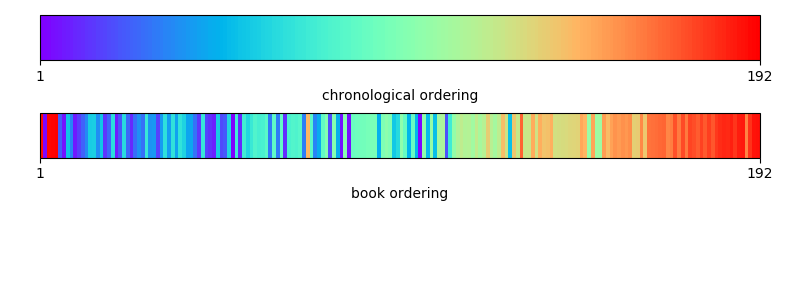
\includegraphics[width=.5\textwidth]{../data/plots/section_bars.png}
    \caption{Contrasting the ordering of events per the book with the chronology presented in \cite{carlisle_2007}}
    \label{chronology_bars}
\end{figure}

\subsubsection{Sierpinski Gasket}

The book's structure is ostensibly based on a Sierpinski Gasket, a triangular fractal.

\begin{figure}[ht]
    \centering
    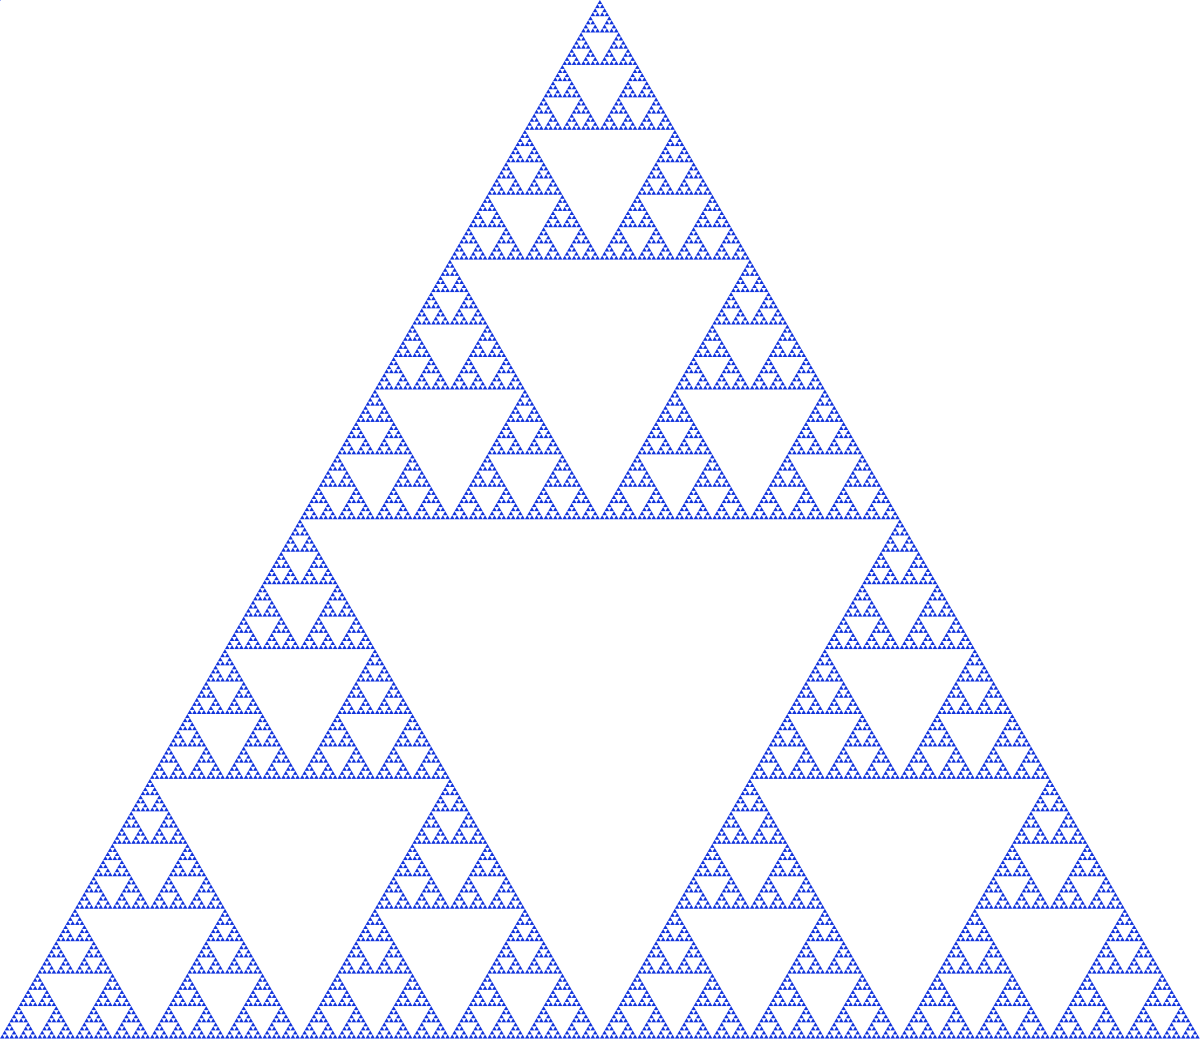
\includegraphics[width=.25\textwidth]{images/sierpinski.png}
    \caption{Sierpinski Gasket}
    \label{Sierpinski Gasket}
\end{figure}

\subsubsection{Endnotes}

The book uses endnotes extensively to convey additional information of varying degrees of relevance. The gamut of information can run from multi-page mini-stories containing important narrative information (\infinitejest, endnote 304) to ``No clue.'' (\infinitejest, endnote 216). Endnotes can reference other endnotes (\infinitejest, endnote 45), and can themselves have endnotes (\infinitejest, endnotes 388). These present a challenge both for the reader and for our approach to generating the network.
